\documentclass[aspectratio=169,11pt,table]{beamer}
\usepackage{../assets/ccde-beamer}

%% ---------- Metadatos (plantilla canónica: \date{} siempre vacío) ----------
\renewcommand{\ccdefootlabel}{CCDE -- Support Vector Machines (SVM)}
\title{Support Vector Machines (SVM)}
\subtitle{Margen máximo, regularización y el método de kernels}
\author{Círculo de Ciencia de Datos y Econometría}
\date{}

\begin{document}


% ================================================================
% Portada canónica (diseño en assets/ccde-beamer.sty, sin fecha)
\ccdeportada{Support Vector Machines (SVM)}{Margen máximo, regularización y el método de kernels}{SVM}


% ================================================================
\begin{frame}{Mapa de la presentación}
\begin{columns}[T,onlytextwidth]
\begin{column}{0.57\textwidth}
\tableofcontents
\end{column}
\begin{column}{0.39\textwidth}
\begin{keybox}
\textbf{Pregunta guía}\\[0.14cm]
¿Cómo construye una SVM una frontera con buena capacidad de generalización y cómo puede volverla no lineal sin trabajar explícitamente en un espacio enorme?
\end{keybox}
\vspace{0.16cm}
\begin{ccdebox}
\small
\textbf{Fuentes troncales}\\
Géron, cap. 5; James et al., cap. 9; Hastie et al., cap. 12.\\[0.12cm]
\textbf{Aplicación}\\
Python + scikit-learn, código reproducible.
\end{ccdebox}
\end{column}
\end{columns}
\end{frame}

% ================================================================

% ================================================================
% SECCIONES MODULARES
% ================================================================
\section{Geometría y margen máximo}

\begin{frame}{¿Qué es una Support Vector Machine?}
\small
\begin{columns}[c,onlytextwidth]
\begin{column}{0.46\textwidth}
\begin{itemize}
  \item Es un método supervisado para \textbf{clasificación}, regresión y detección de novedades.
  \item En clasificación busca una frontera que separe clases con el \textbf{mayor margen posible}.
  \item La frontera queda determinada por unas pocas observaciones críticas: los \textbf{support vectors}.
  \item Con kernels puede construir fronteras no lineales manteniendo un problema de optimización convexo.
\end{itemize}
\end{column}
\begin{column}{0.50\textwidth}
\centering
\begin{tikzpicture}[scale=0.90]
  \draw[->,ccdemid] (-0.5,0) -- (5.6,0) node[right]{\scriptsize $x_1$};
  \draw[->,ccdemid] (0,-0.5) -- (0,4.8) node[above]{\scriptsize $x_2$};
  \foreach \x/\y in {0.8/0.7,1.1/1.7,1.5/1.0,1.8/2.1,2.0/1.4,1.2/2.6}{
    \fill[ccdeaccent] (\x,\y) circle (2.7pt);
  }
  \foreach \x/\y in {3.5/2.2,3.8/3.1,4.2/2.5,4.5/3.7,4.8/2.9,3.9/4.0}{
    \fill[purplex] (\x,\y) circle (2.7pt);
  }
  \draw[ccdenavy,very thick] (0.6,4.2) -- (4.8,0.4);
  \draw[ccdelight,thick,dashed] (0.25,3.55) -- (4.2,-0.02);
  \draw[ccdelight,thick,dashed] (1.25,4.85) -- (5.45,1.05);
  \node[rotate=-42,text=ccdenavy,font=\scriptsize\bfseries] at (3.45,1.95){hiperplano};
  \node[rotate=-42,text=ccdeaccent,font=\scriptsize] at (2.5,3.15){margen};
  \draw[warn,very thick] (2.05,1.42) circle (5pt);
  \draw[warn,very thick] (3.52,2.22) circle (5pt);
  \node[text=warn,font=\scriptsize,align=center] at (4.55,0.65){support\\vectors};
  \draw[->,warn] (4.18,0.95)--(3.67,2.02);
\end{tikzpicture}
\end{column}
\end{columns}
\source{Géron (2022), cap. 5; James et al. (2013), cap. 9.}
\end{frame}

% ================================================================
\begin{frame}{Hiperplano, función de decisión y distancia}
\footnotesize
\begin{columns}[T,onlytextwidth]
\begin{column}{0.52\textwidth}
\begin{ccdebox}
\centering
\textbf{Hiperplano en $\mathbb{R}^p$}
\[
\mathbf{w}^{\top}\mathbf{x}+b=0
\]
\textbf{Regla de clasificación}
\[
\hat y=\operatorname{sign}(\mathbf{w}^{\top}\mathbf{x}+b)
\]
\textbf{Distancia firmada al hiperplano}
\[
\frac{\mathbf{w}^{\top}\mathbf{x}+b}{\|\mathbf{w}\|}
\]
\end{ccdebox}
\end{column}
\begin{column}{0.44\textwidth}
\begin{contrastbox}{ccdeaccent}{Lectura geométrica}
\footnotesize
\begin{itemize}
  \item $\mathbf{w}$ es normal al hiperplano.
  \item $b$ desplaza la frontera.
  \item Escalar $(\mathbf{w},b)$ por la misma constante no cambia la frontera.
  \item Por eso fijamos una escala conveniente para expresar el margen.
\end{itemize}
\end{contrastbox}
\vspace{0.16cm}
\begin{keybox}
La SVM usa esta libertad de escala para imponer que los puntos más cercanos satisfagan $y_i(\mathbf{w}^\top\mathbf{x}_i+b)=1$.
\end{keybox}
\end{column}
\end{columns}
\source{James et al. (2013), secs. 9.1.1--9.1.4; Hastie et al. (2009), cap. 12.}
\end{frame}

% ================================================================
\begin{frame}{¿Por qué maximizar el margen?}
\small
\begin{columns}[c,onlytextwidth]
\begin{column}{0.50\textwidth}
\centering
\begin{tikzpicture}[scale=0.82]
  \draw[->,ccdemid] (-0.3,0)--(5.7,0);
  \draw[->,ccdemid] (0,-0.3)--(0,4.7);
  \foreach \x/\y in {0.8/0.8,1.0/1.9,1.4/1.2,1.6/2.4,2.1/1.8}{\fill[ccdeaccent] (\x,\y) circle(2.5pt);}
  \foreach \x/\y in {3.7/2.1,4.0/3.2,4.4/2.6,4.7/3.7,5.0/3.0}{\fill[purplex] (\x,\y) circle(2.5pt);}
  \draw[warn,thick] (1.1,4.25)--(5.2,0.35);
  \draw[okgreen,very thick] (0.45,4.35)--(4.75,0.28);
  \draw[ccdelight,thick,dashed] (0.05,3.58)--(4.18,-0.28);
  \draw[ccdelight,thick,dashed] (1.15,4.95)--(5.25,1.08);
  \node[text=warn,font=\scriptsize] at (4.45,4.15){separa, pero margen pequeño};
  \node[text=okgreen,font=\scriptsize\bfseries] at (3.90,0.40){margen máximo};
\end{tikzpicture}
\end{column}
\begin{column}{0.46\textwidth}
\begin{itemize}
  \item Si varias fronteras clasifican igual al conjunto de entrenamiento, necesitamos un criterio para elegir una.
  \item La SVM elige el hiperplano que deja la \textbf{calle más ancha} entre las clases.
  \item Con la normalización canónica, la distancia desde la frontera a cada borde del margen es $1/\|\mathbf w\|$.
\end{itemize}
\vspace{0.08cm}
\begin{keybox}[fontupper=\footnotesize]
\centering
\textbf{Ancho total:} $\displaystyle \frac{2}{\|\mathbf w\|}$ \qquad
$\Longrightarrow$ \qquad minimizar $\|\mathbf w\|^2$.
\end{keybox}
\end{column}
\end{columns}
\source{James et al. (2013), sec. 9.1.3; Géron (2022), ``Large Margin Classification''.}
\end{frame}

% ================================================================
\begin{frame}{Hard margin: problema de optimización}
\footnotesize
\begin{columns}[T,onlytextwidth]
\begin{column}{0.55\textwidth}
\begin{ccdebox}
\centering
\textbf{SVM lineal de margen duro}
\[
\min_{\mathbf w,b}\quad \frac{1}{2}\|\mathbf w\|^2
\]
\[
\text{s.a.}\quad y_i(\mathbf w^{\top}\mathbf x_i+b)\ge 1,
\qquad i=1,\dots,n
\]
\end{ccdebox}
\vspace{0.15cm}
\begin{keybox}
Todos los puntos deben quedar del lado correcto y fuera de la franja del margen. No se permite ninguna violación.
\end{keybox}
\end{column}
\begin{column}{0.41\textwidth}
\begin{contrastbox}{ccdeblue}{¿Qué consigue?}
\footnotesize
\begin{itemize}
  \item Separación perfecta, si existe.
  \item Solución de un problema cuadrático convexo.
  \item Óptimo global, no un mínimo local arbitrario.
\end{itemize}
\end{contrastbox}
\vspace{0.16cm}
\begin{contrastbox}{warn}{Condición fuerte}
\footnotesize
Debe existir un hiperplano que separe completamente las clases.
\end{contrastbox}
\end{column}
\end{columns}
\source{Hastie et al. (2009), cap. 12; Géron (2022), apéndice matemático de SVM.}
\end{frame}

% ================================================================
\begin{frame}{Por qué el hard margin suele ser demasiado rígido}
\small
\begin{columns}[T,onlytextwidth]
\begin{column}{0.53\textwidth}
\IfFileExists{fig_svm_hard_soft.png}{%
  \centering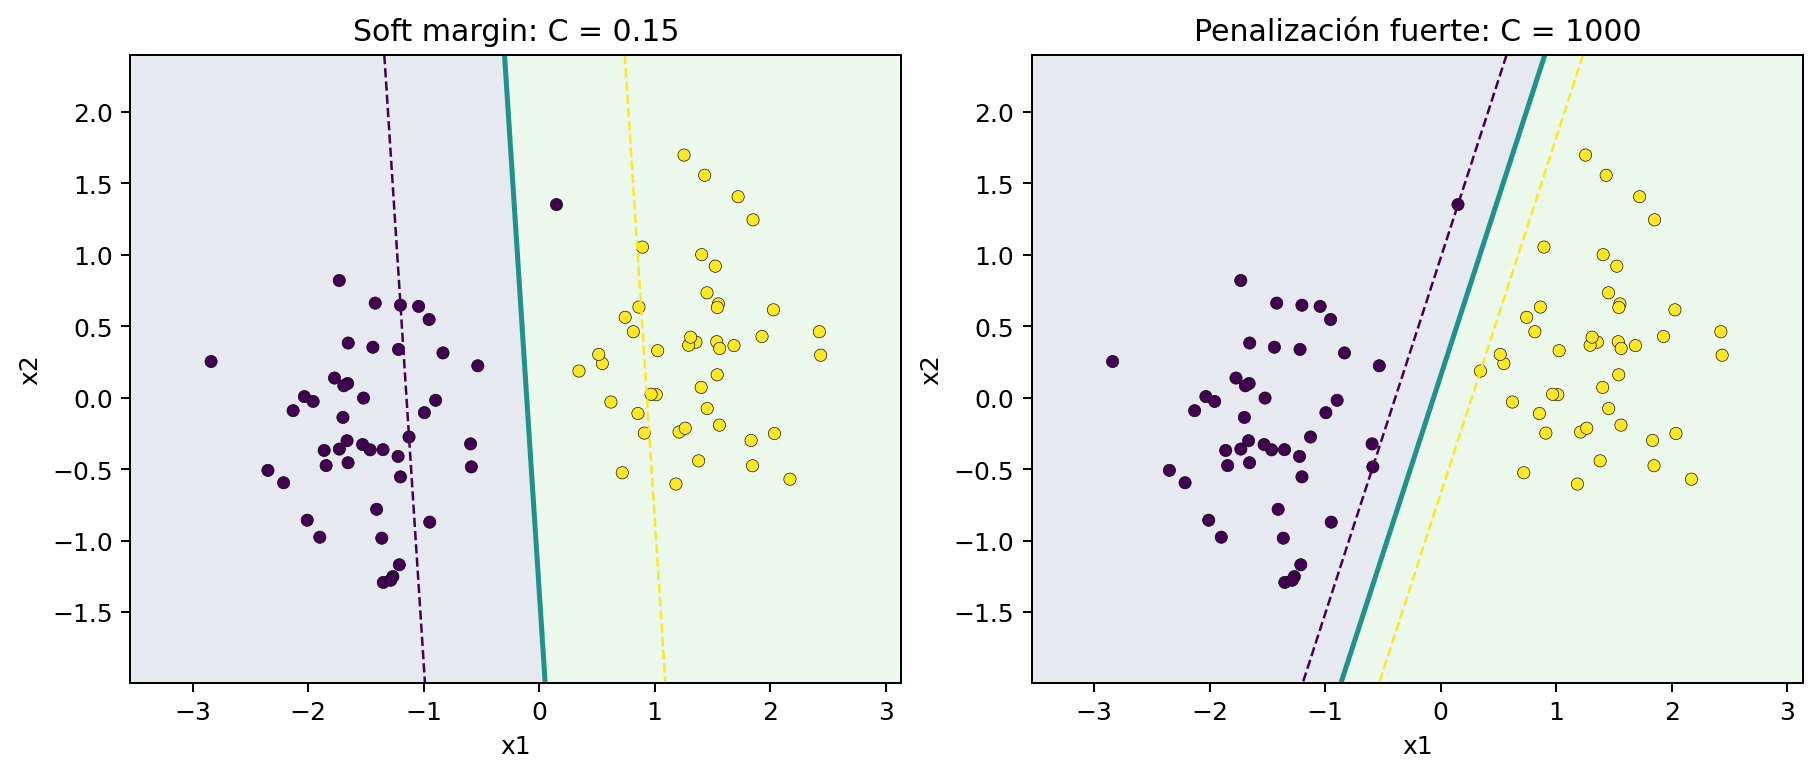
\includegraphics[width=\linewidth]{fig_svm_hard_soft.png}
}{%
  \begin{ccdebox}\centering\small Ejecuta \texttt{python codigo\_demo\_svm.py} para generar la figura comparativa.\end{ccdebox}}
\end{column}
\begin{column}{0.43\textwidth}
\begin{contrastbox}{warn}{Problema 1: separabilidad}
\small
Si las clases se solapan, el conjunto de restricciones del hard margin puede ser imposible.
\end{contrastbox}
\vspace{0.16cm}
\begin{contrastbox}{warn}{Problema 2: outliers}
\small
Una sola observación extrema puede mover drásticamente la frontera para conservar separación perfecta.
\end{contrastbox}
\vspace{0.16cm}
\begin{keybox}
Necesitamos permitir errores controlados: eso conduce al \textbf{soft margin}.
\end{keybox}
\end{column}
\end{columns}
\source{Géron (2022), ``Soft Margin Classification''. Figura generada por \texttt{codigo\_demo\_svm.py}.}
\end{frame}

% ================================================================

\section{Soft margin y regularización}

\begin{frame}{Soft margin: permitir violaciones con variables de holgura}
\footnotesize
\begin{columns}[T,onlytextwidth]
\begin{column}{0.56\textwidth}
\begin{ccdebox}
\centering
\textbf{Formulación primal usada por scikit-learn}
\[
\min_{\mathbf w,b,\boldsymbol\xi}
\quad
\frac{1}{2}\|\mathbf w\|^2
+ C\sum_{i=1}^{n}\xi_i
\]
\[
\text{s.a.}\quad
 y_i(\mathbf w^\top\mathbf x_i+b)\ge 1-\xi_i,
\qquad \xi_i\ge 0
\]
\end{ccdebox}
\vspace{0.12cm}
\begin{keybox}
$\xi_i$ mide cuánto puede violar el margen la observación $i$; si cruza la frontera, la violación es aún mayor.
\end{keybox}
\end{column}
\begin{column}{0.40\textwidth}
\begin{contrastbox}{ccdeaccent}{Dos objetivos en tensión}
\footnotesize
\begin{enumerate}
  \item Margen grande: minimizar $\|\mathbf w\|^2$.
  \item Pocas violaciones: minimizar $\sum_i \xi_i$.
\end{enumerate}
\end{contrastbox}
\vspace{0.14cm}
\begin{contrastbox}{ccdeblue}{El papel de $C$}
\footnotesize
$C$ decide cuánto penalizamos las violaciones frente a la anchura del margen.
\end{contrastbox}
\end{column}
\end{columns}
\source{Géron (2022), ``Soft Margin Classification'' y Eq. 5-2.}
\end{frame}

% ================================================================
\begin{frame}{$C$ controla el trade-off sesgo--varianza}
\small
\begin{columns}[T,onlytextwidth]
\begin{column}{0.47\textwidth}
\begin{contrastbox}{ccdeaccent}{En scikit-learn: $C$ pequeño}
\small
\begin{itemize}
  \item Más regularización.
  \item Margen más ancho.
  \item Tolera más violaciones.
  \item Menor varianza, más riesgo de underfitting.
\end{itemize}
\end{contrastbox}
\end{column}
\begin{column}{0.47\textwidth}
\begin{contrastbox}{warn}{En scikit-learn: $C$ grande}
\small
\begin{itemize}
  \item Menos regularización.
  \item Penaliza fuertemente violaciones.
  \item Frontera más ajustada a la muestra.
  \item Menor sesgo, más riesgo de overfitting.
\end{itemize}
\end{contrastbox}
\end{column}
\end{columns}
\vspace{0.22cm}
\begin{keybox}
\textbf{Cuidado con la notación:} ISLR (James et al.) usa otra parametrización de $C$ como presupuesto de violaciones, por lo que allí un $C$ mayor implica un margen más ancho. En scikit-learn y en Géron, $C$ es la penalización de las violaciones y la relación es la contraria.
\end{keybox}
\source{Géron (2022), cap. 5; James et al. (2013), sec. 9.2.2.}
\end{frame}

% ================================================================
\begin{frame}{Support vectors: los puntos que realmente fijan la frontera}
\small
\begin{columns}[c,onlytextwidth]
\begin{column}{0.50\textwidth}
\centering
\begin{tikzpicture}[scale=0.86]
  \draw[ccdelight,thick,dashed] (0.1,3.3)--(4.6,-0.2);
  \draw[ccdenavy,very thick] (0.65,4.05)--(5.15,0.55);
  \draw[ccdelight,thick,dashed] (1.2,4.8)--(5.7,1.3);
  \foreach \x/\y in {0.6/0.7,1.0/1.2,1.3/2.2,1.8/1.5,2.0/2.7}{\fill[ccdeaccent] (\x,\y) circle(2.6pt);}
  \foreach \x/\y in {3.5/2.1,4.0/3.0,4.4/2.7,4.7/3.6,5.0/4.1}{\fill[purplex] (\x,\y) circle(2.6pt);}
  \draw[warn,very thick] (2.02,2.68) circle(6pt);
  \draw[warn,very thick] (3.48,2.12) circle(6pt);
  \draw[warn,very thick] (1.34,2.19) circle(6pt);
  \node[text=warn,font=\scriptsize\bfseries] at (4.2,0.35){puntos activos};
  \draw[->,warn] (3.9,0.65)--(3.48,1.9);
\end{tikzpicture}
\end{column}
\begin{column}{0.46\textwidth}
\begin{itemize}
  \item Son observaciones sobre el margen, dentro del margen o mal clasificadas.
  \item En la solución dual tienen multiplicadores $\alpha_i>0$.
  \item Observaciones suficientemente alejadas del margen tienen $\alpha_i=0$.
  \item Por ello la función de decisión depende de un subconjunto de entrenamiento.
\end{itemize}
\vspace{0.14cm}
\begin{keybox}
Esta \textbf{esparsidad} es una propiedad importante: los puntos lejanos a la frontera no cambian la solución directamente.
\end{keybox}
\end{column}
\end{columns}
\source{James et al. (2013), secs. 9.1.3 y 9.2; Hastie et al. (2009), cap. 12.}
\end{frame}

% ================================================================

\section{Dualidad y kernels}

\begin{frame}{La formulación dual revela dónde entra el kernel}
\scriptsize
\begin{columns}[T,onlytextwidth]
\begin{column}{0.58\textwidth}
\begin{ccdebox}
\centering
\textbf{Problema dual del soft-margin SVM}
\[
\max_{\boldsymbol\alpha}
\quad
\sum_{i=1}^{n}\alpha_i
-\frac12\sum_{i=1}^{n}\sum_{j=1}^{n}
\alpha_i\alpha_j y_i y_j
\underbrace{\mathbf x_i^\top\mathbf x_j}_{\text{producto interno}}
\]
\[
\text{s.a.}\quad
0\le \alpha_i\le C,
\qquad
\sum_{i=1}^{n}\alpha_i y_i=0
\]
\end{ccdebox}
\vspace{0.12cm}
\begin{keybox}[fontupper=\footnotesize]
La optimización ya no necesita las coordenadas por separado: solo aparecen productos internos entre pares de observaciones.
\end{keybox}
\end{column}
\begin{column}{0.38\textwidth}
\begin{contrastbox}{ccdeaccent}{Consecuencia}
\footnotesize
Si reemplazamos
\[
\mathbf x_i^\top\mathbf x_j
\quad\text{por}\quad
K(\mathbf x_i,\mathbf x_j),
\]
obtenemos un clasificador lineal en otro espacio de características sin tener que construirlo explícitamente.
\end{contrastbox}
\end{column}
\end{columns}
\source{Hastie et al. (2009), cap. 12; Géron (2022), ``The Dual Problem'' y ``Kernelized SVMs''.}
\end{frame}

% ================================================================
\begin{frame}{Cambio de dimensionalidad: una frontera no lineal puede volverse lineal}
\small
\begin{columns}[c,onlytextwidth]
\begin{column}{0.38\textwidth}
\centering
\textbf{Espacio original: 1D}\\[0.15cm]
\begin{tikzpicture}[x=0.82cm,y=0.82cm]
  \draw[->,ccdemid] (-3.5,0)--(3.7,0) node[right]{\scriptsize $x$};
  \foreach \x in {-3,-2.4,2.4,3}{\fill[purplex] (\x,0) circle(3pt);}
  \foreach \x in {-0.9,-0.4,0,0.5,1.0}{\fill[ccdeaccent] (\x,0) circle(3pt);}
  \node[text=purplex,font=\scriptsize] at (0,1.0){clase $+1$ en ambos extremos};
  \node[text=ccdeaccent,font=\scriptsize] at (0,-0.9){clase $-1$ en el centro};
\end{tikzpicture}
\vspace{0.20cm}
\begin{contrastbox}{warn}{No separable con un umbral}
\scriptsize
Una sola frontera lineal en 1D es un punto; no puede dejar $+1$ en ambos extremos y $-1$ en el centro.
\end{contrastbox}
\end{column}
\begin{column}{0.12\textwidth}
\centering
\Huge\textcolor{ccdeaccent}{$\Longrightarrow$}\\[-0.05cm]
\scriptsize $\phi(x)=(x,x^2)$
\end{column}
\begin{column}{0.46\textwidth}
\centering
\textbf{Espacio transformado: 2D}\\[0.10cm]
\begin{tikzpicture}[x=0.70cm,y=0.60cm]
  \draw[->,ccdemid] (-3.6,0)--(3.7,0) node[right]{\scriptsize $x$};
  \draw[->,ccdemid] (0,-0.3)--(0,5.0) node[above]{\scriptsize $x^2$};
  \draw[ccdemid!60,thin,domain=-3.1:3.1,samples=80] plot (\x,{0.48*\x*\x});
  \foreach \x in {-3,-2.4,2.4,3}{\fill[purplex] (\x,{0.48*\x*\x}) circle(3pt);}
  \foreach \x in {-0.9,-0.4,0,0.5,1.0}{\fill[ccdeaccent] (\x,{0.48*\x*\x}) circle(3pt);}
  \draw[okgreen,very thick] (-3.3,2.35)--(3.3,2.35);
  \node[text=okgreen,font=\scriptsize\bfseries] at (2.0,2.70){hiperplano lineal};
\end{tikzpicture}
\vspace{0.08cm}
\begin{keybox}[fontupper=\scriptsize]
Una frontera lineal en el espacio ampliado se proyecta como una frontera \textbf{no lineal} en el espacio original.
\end{keybox}
\end{column}
\end{columns}
\source{Intuición de expansión de bases: James et al. (2013), sec. 9.3; Hastie et al. (2009), secs. 12.3 y 12.4.}
\end{frame}

% ================================================================
\begin{frame}{El kernel trick: calcular similitudes sin construir $\phi(x)$}
\footnotesize
\begin{columns}[T,onlytextwidth]
\begin{column}{0.52\textwidth}
\begin{ccdebox}
\centering
Supongamos una transformación potencialmente enorme:
\[
\phi:\mathbb R^p\to\mathcal H
\]
Un kernel válido satisface
\[
\boxed{K(\mathbf x,\mathbf z)=\langle \phi(\mathbf x),\phi(\mathbf z)\rangle_{\mathcal H}}
\]
La SVM solo necesita esos productos internos.
\end{ccdebox}
\vspace{0.14cm}
\begin{keybox}
No calculamos todas las nuevas variables. Construimos la matriz de Gram $K_{ij}=K(\mathbf x_i,\mathbf x_j)$ y optimizamos con ella.
\end{keybox}
\end{column}
\begin{column}{0.44\textwidth}
\begin{contrastbox}{ccdeaccent}{Por qué es potente}
\footnotesize
\begin{itemize}
  \item Un kernel polinómico equivale a usar interacciones y potencias.
  \item El RBF corresponde a un espacio de características implícito de dimensión infinita.
  \item El costo depende de evaluar $K$, no de materializar ese espacio.
\end{itemize}
\end{contrastbox}
\vspace{0.14cm}
\begin{contrastbox}{ccdeblue}{Condición matemática}
\footnotesize
Para kernels estándar, la matriz de Gram debe ser simétrica y semidefinida positiva; así puede interpretarse como un producto interno en algún espacio de Hilbert.
\end{contrastbox}
\end{column}
\end{columns}
\source{James et al. (2013), sec. 9.3; Hastie et al. (2009), secs. 12.3.3 y 12.3.7.}
\end{frame}

% ================================================================
\begin{frame}{Kernels más usados}
\scriptsize
\renewcommand{\arraystretch}{1.45}
\setlength{\tabcolsep}{5.0pt}
\begin{center}
\begin{tabular}{p{2.2cm}p{5.0cm}p{5.0cm}}
\toprule
\rowcolor{ccdenavy}
\textcolor{white}{\textbf{Kernel}} &
\textcolor{white}{\textbf{Fórmula}} &
\textcolor{white}{\textbf{Intuición / hiperparámetros}}\\
\midrule
Lineal & $K(x,z)=x^\top z$ & Sin expansión no lineal; suele funcionar bien cuando $p$ es grande.\\
\rowcolor{ccdeice!50}
Polinómico & $K(x,z)=(\gamma x^\top z+r)^d$ & $d$ controla grado; $\gamma$ escala la similitud; $r=\texttt{coef0}$ cambia peso entre términos de distinto orden.\\
RBF / Gaussiano & $K(x,z)=\exp(-\gamma\|x-z\|^2)$ & Similitud local. $\gamma$ alto: influencia muy local; $\gamma$ bajo: frontera más suave.\\
\rowcolor{ccdeice!50}
Sigmoide & $K(x,z)=\tanh(\gamma x^\top z+r)$ & Menos común; se parece formalmente a una neurona sigmoide.\\
\bottomrule
\end{tabular}
\end{center}
\vspace{0.16cm}
\begin{keybox}
En práctica, la comparación más importante suele ser \textbf{lineal vs. RBF}; los hiperparámetros deben elegirse con validación cruzada, no por ajuste visual al training set.
\end{keybox}
\source{James et al. (2013), Eqs. 9.22--9.24; Géron (2022), ``Polynomial Kernel'' y ``Gaussian RBF Kernel''.}
\end{frame}

% ================================================================
\begin{frame}{RBF en profundidad: $\gamma$ define el radio de influencia}
\small
\begin{columns}[T,onlytextwidth]
\begin{column}{0.66\textwidth}
\IfFileExists{fig_svm_gamma.png}{%
  \centering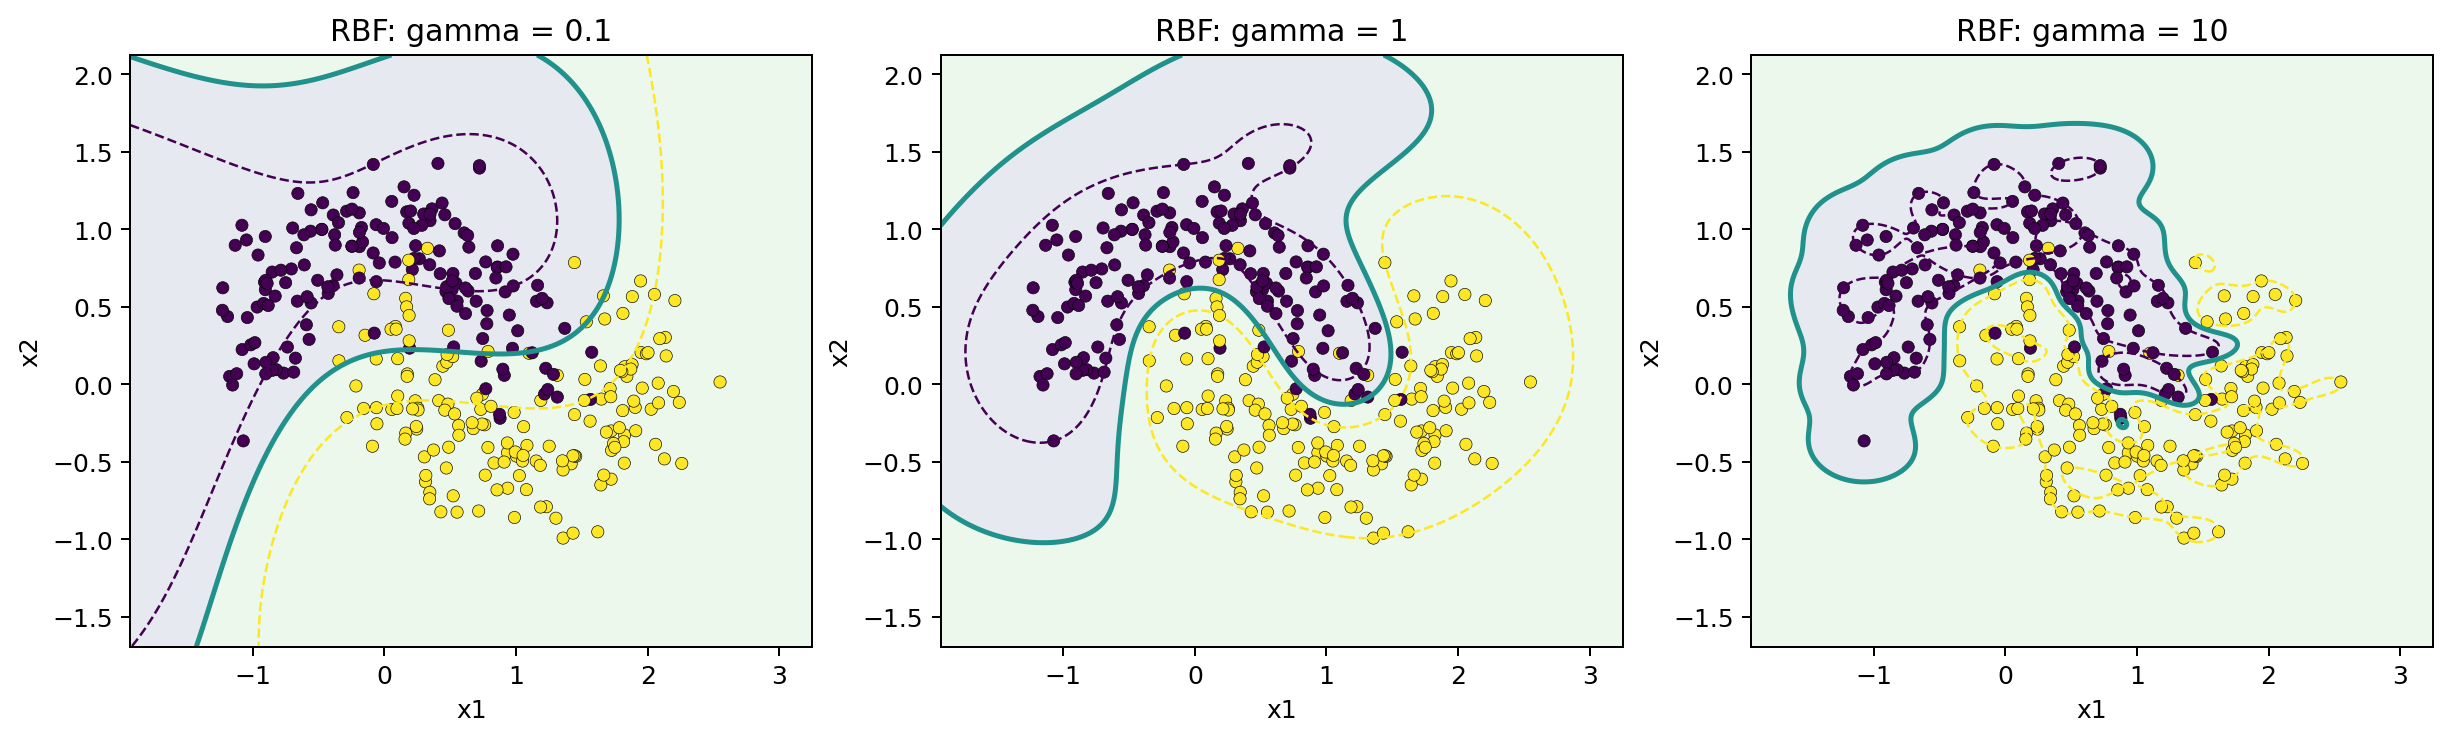
\includegraphics[width=\linewidth]{fig_svm_gamma.png}
}{%
  \begin{ccdebox}\centering\small Ejecuta \texttt{python codigo\_demo\_svm.py} para generar la figura de $\gamma$.\end{ccdebox}}
\end{column}
\begin{column}{0.30\textwidth}
\begin{contrastbox}{ccdeblue}{$\gamma$ bajo}
\scriptsize
La similitud cae lentamente con la distancia. Cada punto influye sobre una región grande: frontera suave, mayor sesgo.
\end{contrastbox}
\vspace{0.10cm}
\begin{contrastbox}{warn}{$\gamma$ alto}
\scriptsize
La similitud cae muy rápido. Cada punto influye localmente: frontera ondulada, mayor varianza.
\end{contrastbox}
\end{column}
\end{columns}
\source{Géron (2022), Figura 5-9; James et al. (2013), Eq. 9.24. Figura generada localmente.}
\end{frame}

% ================================================================
\begin{frame}{La función de decisión kernelizada}
\footnotesize
\begin{columns}[T,onlytextwidth]
\begin{column}{0.56\textwidth}
\begin{ccdebox}
\centering
Después de resolver el dual:
\[
f(\mathbf x)=
\sum_{i\in SV}\alpha_i y_i K(\mathbf x_i,\mathbf x)+b
\]
\[
\hat y=\operatorname{sign}(f(\mathbf x))
\]
\end{ccdebox}
\vspace{0.12cm}
\begin{keybox}
Solo aparecen los support vectors: aquellos con $\alpha_i>0$. Para un RBF, los support vectors cercanos a $x$ reciben mayor similitud y pesan más en la decisión.
\end{keybox}
\end{column}
\begin{column}{0.40\textwidth}
\begin{contrastbox}{ccdeaccent}{Lectura operacional}
\footnotesize
Para predecir una nueva observación:
\begin{enumerate}
  \item medir su similitud con cada support vector;
  \item ponderar por $\alpha_i y_i$;
  \item sumar el intercepto $b$;
  \item tomar el signo.
\end{enumerate}
\end{contrastbox}
\end{column}
\end{columns}
\source{James et al. (2013), Eq. 9.23; Hastie et al. (2009), cap. 12.}
\end{frame}

% ================================================================

\section{Hiperparámetros y uso práctico}

\begin{frame}{Hiperparámetros principales en \texttt{sklearn.svm.SVC}}
\scriptsize
\renewcommand{\arraystretch}{1.40}
\setlength{\tabcolsep}{4.6pt}
\begin{center}
\begin{tabular}{p{2.05cm}p{4.0cm}p{6.15cm}}
\toprule
\rowcolor{ccdenavy}
\textcolor{white}{\textbf{Parámetro}} &
\textcolor{white}{\textbf{Actúa sobre}} &
\textcolor{white}{\textbf{Qué ocurre al modificarlo}}\\
\midrule
\texttt{C} & Regularización / penalización & Mayor $C$: menos tolerancia a violaciones; menor $C$: margen más ancho y más regularización.\\
\rowcolor{ccdeice!50}
\texttt{kernel} & Geometría de la frontera & \texttt{linear}, \texttt{rbf}, \texttt{poly}, \texttt{sigmoid} o función propia.\\
\texttt{gamma} & Escala del RBF/poly/sigmoid & Alto: influencia local y mayor flexibilidad. Bajo: frontera más suave. \texttt{scale} usa una regla basada en varianza.\\
\rowcolor{ccdeice!50}
\texttt{degree} & Kernel polinómico & Grado $d$; solo importa con \texttt{poly}.\\
\texttt{coef0} & Poly / sigmoid & Término independiente $r$; altera peso relativo de términos de orden alto y bajo.\\
\rowcolor{ccdeice!50}
\texttt{class\_weight} & Costos por clase & Útil con desbalance: permite penalizar más errores de una clase.\\
\bottomrule
\end{tabular}
\end{center}
\source{Géron (2022), cap. 5; API conceptual de SVC usada en el código asociado.}
\end{frame}

% ================================================================
\begin{frame}{Escalar variables no es opcional en SVM}
\small
\begin{columns}[T,onlytextwidth]
\begin{column}{0.46\textwidth}
\begin{contrastbox}{warn}{Sin escalamiento}
\small
Si una variable está en miles y otra entre 0 y 1, las distancias y productos internos quedan dominados por la primera.
\end{contrastbox}
\vspace{0.14cm}
\begin{contrastbox}{ccdeaccent}{Con \texttt{StandardScaler}}
\small
Las variables se centran y escalan antes de estimar la SVM. Para evitar fuga de información, el escalamiento debe vivir dentro de un \texttt{Pipeline}.
\end{contrastbox}
\end{column}
\begin{column}{0.50\textwidth}
\centering
\begin{tikzpicture}[scale=0.88]
\node[draw,rounded corners,fill=white,minimum width=3.2cm,minimum height=0.75cm] (raw) at (0,2.8) {datos crudos};
\node[draw,rounded corners,fill=ccdeice,minimum width=3.2cm,minimum height=0.75cm] (scale) at (0,1.45) {\texttt{StandardScaler}};
\node[draw,rounded corners,fill=ccdelight!22,minimum width=3.2cm,minimum height=0.75cm] (svc) at (0,0.1) {\texttt{SVC}};
\node[draw,rounded corners,fill=white,minimum width=3.2cm,minimum height=0.75cm] (pred) at (0,-1.25) {predicción};
\foreach \a/\b in {raw/scale,scale/svc,svc/pred}{\draw[->,thick,ccdeaccent](\a)--(\b);}
\node[text=ccdemid,font=\scriptsize,align=center] at (4.15,1.45){fit del scaler\\solo con training};
\draw[->,ccdemid] (3.3,1.45)--(1.7,1.45);
\end{tikzpicture}
\end{column}
\end{columns}
\source{Géron (2022), Figura 5-2 y ejemplo de pipeline con \texttt{StandardScaler}.}
\end{frame}

% ================================================================
\begin{frame}{Cómo ajustar $C$ y $\gamma$ sin engañarnos}
\small
\begin{columns}[T,onlytextwidth]
\begin{column}{0.49\textwidth}
\begin{contrastbox}{ccdeblue}{Flujo recomendado}
\small
\begin{enumerate}
  \item Separar train y test.
  \item Pipeline: escalamiento + SVC.
  \item Validación cruzada dentro de train.
  \item Explorar escala logarítmica para $C$ y $\gamma$.
  \item Elegir por una métrica coherente con el problema.
  \item Evaluar una sola vez en test.
\end{enumerate}
\end{contrastbox}
\end{column}
\begin{column}{0.47\textwidth}
\begin{keybox}
\textbf{Ejemplo de grilla}
\[
C\in\{0.1,1,10,100\}
\]
\[
\gamma\in\{0.1,1,10,\texttt{scale}\}
\]
\end{keybox}
\vspace{0.14cm}
\begin{ccdebox}
\small
En clasificación desbalanceada, accuracy puede ser pobre criterio. Considerar ROC-AUC, PR-AUC, recall, precision y costos de error.
\end{ccdebox}
\end{column}
\end{columns}
\source{Géron (2022), selección de modelos y cap. 5; James et al. (2013), sec. 9.6.2.}
\end{frame}

% ================================================================
\begin{frame}{Ventajas y desventajas}
\footnotesize
\begin{columns}[T,onlytextwidth]
\begin{column}{0.47\textwidth}
\begin{contrastbox}{ccdeaccent}{Ventajas}
\footnotesize
\begin{itemize}
  \item Excelente capacidad predictiva en datos pequeños/medianos.
  \item Muy útil en alta dimensión, incluso con $p\gg n$.
  \item Kernels capturan fronteras no lineales complejas.
  \item Problema convexo: solución global.
  \item Solo support vectors fijan la frontera.
  \item Regularización explícita mediante $C$.
\end{itemize}
\end{contrastbox}
\end{column}
\begin{column}{0.47\textwidth}
\begin{contrastbox}{warn}{Desventajas}
\footnotesize
\begin{itemize}
  \item No escala bien a conjuntos muy grandes, especialmente SVC kernelizado.
  \item Sensible al escalamiento de variables.
  \item $C$ y $\gamma$ pueden exigir búsqueda cuidadosa.
  \item Menos interpretable que modelos lineales o árboles simples.
  \item Predicciones probabilísticas no son nativas.
  \item Elegir un kernel inadecuado puede aumentar mucho sesgo o varianza.
\end{itemize}
\end{contrastbox}
\end{column}
\end{columns}
\source{Géron (2022), introducción del cap. 5; James et al. (2013), cap. 9.}
\end{frame}

% ================================================================
\begin{frame}{¿Cuándo elegir una SVM?}
\footnotesize
\begin{columns}[T,onlytextwidth]
\begin{column}{0.31\textwidth}
\begin{ccdebox}
\centering
\textbf{Alta dimensión}\\[0.12cm]
Texto, genómica, muchas variables respecto al número de observaciones. Un kernel lineal puede ser suficiente.
\end{ccdebox}
\end{column}
\begin{column}{0.31\textwidth}
\begin{ccdebox}
\centering
\textbf{Frontera no lineal}\\[0.12cm]
Cuando un modelo lineal falla y el tamaño muestral permite trabajar con RBF o polinómico.
\end{ccdebox}
\end{column}
\begin{column}{0.31\textwidth}
\begin{ccdebox}
\centering
\textbf{Precisión > explicación}\\[0.12cm]
Cuando importa más una frontera robusta que una interpretación directa de coeficientes.
\end{ccdebox}
\end{column}
\end{columns}
\vspace{0.22cm}
\begin{keybox}
\textbf{No es primera opción} para millones de observaciones con kernel RBF. En ese caso conviene comparar con modelos lineales escalables, árboles/boosting o aproximaciones al kernel.
\end{keybox}
\source{Géron (2022), cap. 5; James et al. (2013), aplicación de expresión génica en sec. 9.6.5.}
\end{frame}

% ================================================================

\section{Aplicación en Python}

\begin{frame}{Ejemplo visual: lineal vs. RBF sobre una frontera curva}
\small
\begin{columns}[T,onlytextwidth]
\begin{column}{0.66\textwidth}
\IfFileExists{fig_svm_kernel_moons.png}{%
  \centering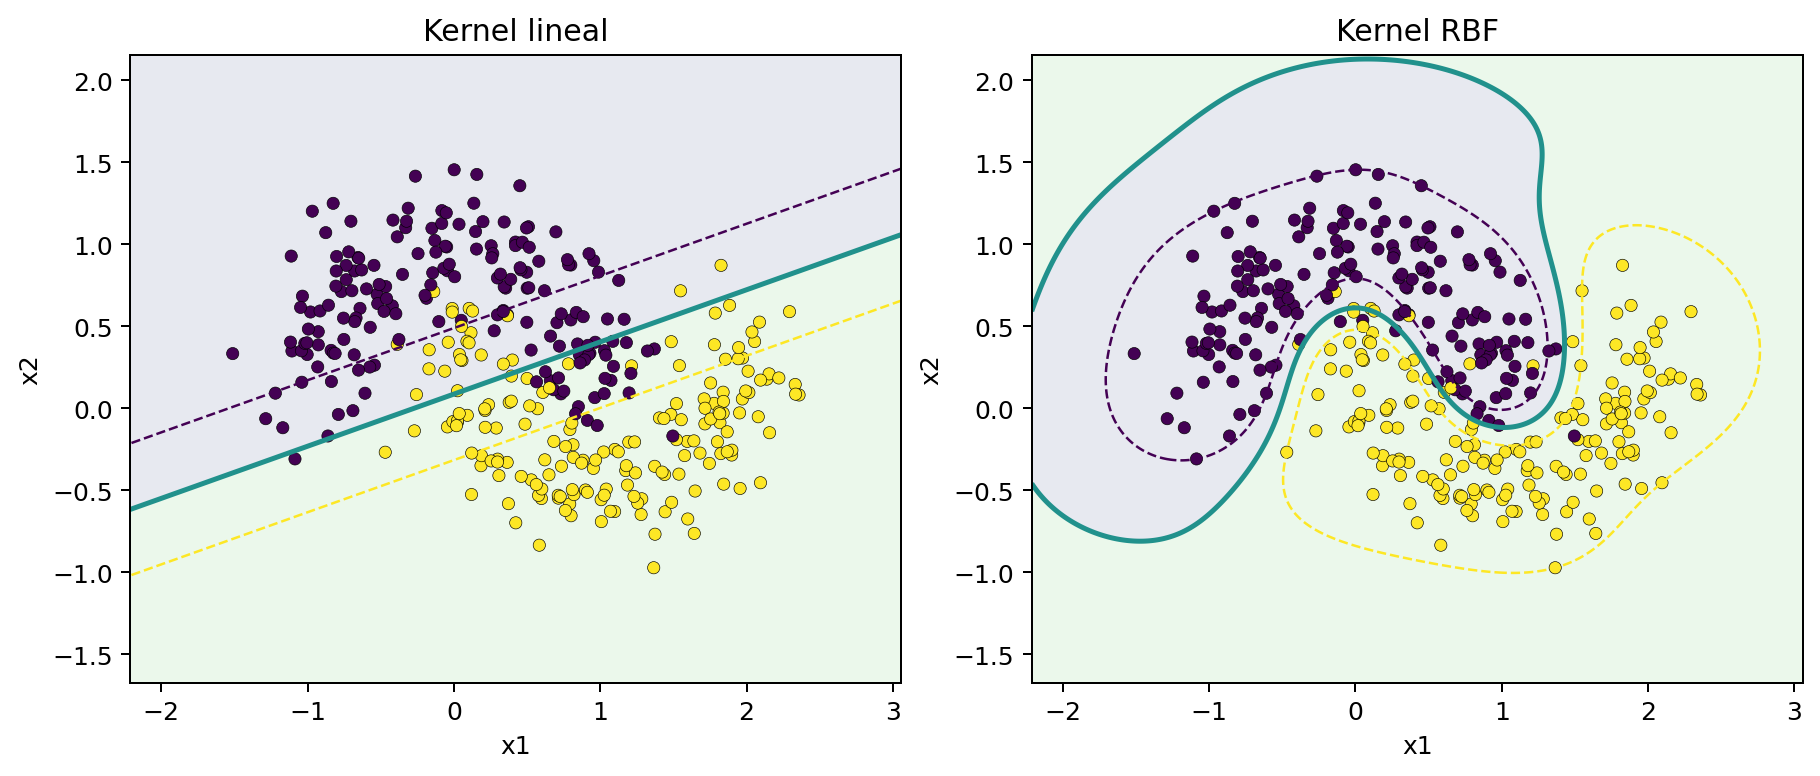
\includegraphics[width=\linewidth]{fig_svm_kernel_moons.png}
}{%
  \begin{ccdebox}\centering\small Ejecuta \texttt{python codigo\_demo\_svm.py} para generar esta comparación.\end{ccdebox}}
\end{column}
\begin{column}{0.30\textwidth}
\begin{contrastbox}{ccdeblue}{Kernel lineal}
\scriptsize
Solo puede construir un hiperplano en el espacio original. Con \texttt{make\_moons} queda sesgado.
\end{contrastbox}
\vspace{0.11cm}
\begin{contrastbox}{ccdeaccent}{Kernel RBF}
\scriptsize
Construye una separación curvada mediante similitudes locales en el espacio implícito.
\end{contrastbox}
\vspace{0.11cm}
\begin{keybox}[fontupper=\scriptsize]
La flexibilidad adicional debe validarse fuera de muestra.
\end{keybox}
\end{column}
\end{columns}
\source{Figura generada por \texttt{codigo\_demo\_svm.py}, semilla 42.}
\end{frame}

% ================================================================
\begin{frame}[fragile]{Python 1/3: pipeline y separación train/test}
\scriptsize
\begin{columns}[T,onlytextwidth]
\begin{column}{0.64\textwidth}
\begin{lstlisting}[style=ccdepython]
from sklearn.datasets import make_moons
from sklearn.model_selection import train_test_split
from sklearn.pipeline import make_pipeline
from sklearn.preprocessing import StandardScaler
from sklearn.svm import SVC

X, y = make_moons(
    n_samples=600, noise=0.25, random_state=42
)
X_train, X_test, y_train, y_test = train_test_split(
    X, y, test_size=0.30,
    stratify=y, random_state=42
)

model = make_pipeline(
    StandardScaler(),
    SVC(kernel="rbf", C=10, gamma="scale")
)
model.fit(X_train, y_train)
\end{lstlisting}
\end{column}
\begin{column}{0.32\textwidth}
\begin{keybox}
\textbf{Puntos clave}
\begin{itemize}
  \item Escalamiento dentro del pipeline.
  \item \texttt{stratify} conserva proporciones.
  \item Semilla fija para reproducibilidad.
  \item RBF para una frontera no lineal.
\end{itemize}
\end{keybox}
\end{column}
\end{columns}
\end{frame}

% ================================================================
\begin{frame}[fragile]{Python 2/3: validación cruzada de $C$, $\gamma$ y kernel}
\scriptsize
\begin{columns}[T,onlytextwidth]
\begin{column}{0.67\textwidth}
\begin{lstlisting}[style=ccdepython]
from sklearn.model_selection import GridSearchCV

pipe = make_pipeline(StandardScaler(), SVC())
param_grid = [
    {
        "svc__kernel": ["linear"],
        "svc__C": [0.1, 1, 10, 100],
    },
    {
        "svc__kernel": ["rbf"],
        "svc__C": [0.1, 1, 10, 100],
        "svc__gamma": ["scale", 0.1, 1, 10],
    },
]

search = GridSearchCV(
    pipe, param_grid, scoring="roc_auc",
    cv=5, n_jobs=-1, refit=True
)
search.fit(X_train, y_train)
\end{lstlisting}
\end{column}
\begin{column}{0.29\textwidth}
\begin{keybox}
\textbf{Por qué así}
\begin{itemize}
  \item La grilla vive solo en training.
  \item Escalamiento se re-estima en cada fold.
  \item Se compara lineal vs. RBF.
  \item ROC-AUC guía la selección.
\end{itemize}
\end{keybox}
\end{column}
\end{columns}
\end{frame}

% ================================================================
\begin{frame}[fragile]{Python 3/3: evaluación fuera de muestra}
\scriptsize
\begin{columns}[T,onlytextwidth]
\begin{column}{0.65\textwidth}
\begin{lstlisting}[style=ccdepython]
from sklearn.metrics import (
    accuracy_score, confusion_matrix, roc_auc_score
)

best = search.best_estimator_
pred = best.predict(X_test)
score = best.decision_function(X_test)

print(search.best_params_)
print("accuracy =", accuracy_score(y_test, pred))
print("roc_auc =", roc_auc_score(y_test, score))
print(confusion_matrix(y_test, pred))
print(
    "support vectors =",
    best.named_steps["svc"].n_support_
)
\end{lstlisting}
\end{column}
\begin{column}{0.31\textwidth}
\begin{contrastbox}{ccdeaccent}{Resultado reproducible}
\scriptsize
Mejor grilla: RBF, $C=10$, $\gamma=\texttt{scale}$.\\[0.10cm]
ROC-AUC CV: \textbf{0.9724}.\\
Accuracy test: \textbf{0.9167}.\\
ROC-AUC test: \textbf{0.9817}.\\
Support vectors: $42+39=81$.
\end{contrastbox}
\end{column}
\end{columns}
\source{Ejecución local de \texttt{codigo\_demo\_svm.py}; scikit-learn, semilla 42.}
\end{frame}

% ================================================================
\begin{frame}{Lineal vs. RBF: resultado del mismo experimento}
\begin{columns}[T,onlytextwidth]
\begin{column}{0.58\textwidth}
\vspace{1.55cm}
\renewcommand{\arraystretch}{1.45}
\small
\begin{tabular}{lccc}
\toprule
\rowcolor{ccdenavy}
\textcolor{white}{\textbf{Modelo}} &
\textcolor{white}{\textbf{Accuracy}} &
\textcolor{white}{\textbf{ROC-AUC}} &
\textcolor{white}{\textbf{SV}}\\
\midrule
SVM lineal & 0.8556 & 0.9383 & 141\\
\rowcolor{ccdeice!50}
SVM RBF & \textbf{0.9333} & \textbf{0.9775} & 75\\
\bottomrule
\end{tabular}
\end{column}
\begin{column}{0.38\textwidth}
\begin{keybox}
\textbf{Lectura}
\begin{itemize}
  \item La estructura de \texttt{make\_moons} es no lineal.
  \item El RBF reduce el sesgo respecto al hiperplano lineal.
  \item Menos support vectors no implica siempre mejor modelo, pero aquí la frontera RBF es además más parsimoniosa en puntos activos.
\end{itemize}
\end{keybox}
\end{column}
\end{columns}
\source{Ejecución de \texttt{codigo\_demo\_svm.py}, semilla 42.}
\end{frame}

% ================================================================

\section{Cierre y fuentes}

\begin{frame}{Ideas que deben quedar}
\footnotesize
\begin{columns}[T,onlytextwidth]
\begin{column}{0.60\textwidth}
\begin{enumerate}
  \item Una SVM lineal busca el hiperplano con máximo margen.
  \item Hard margin exige separación perfecta; soft margin introduce holguras y regularización.
  \item En scikit-learn, $C$ alto penaliza más los errores; $C$ bajo regulariza más.
  \item La formulación dual depende de productos internos, lo que habilita kernels.
  \item El kernel trick equivale a trabajar en un espacio de características ampliado sin construirlo explícitamente.
  \item En RBF, $\gamma$ gobierna la localidad; $C$ y $\gamma$ deben validarse conjuntamente, siempre dentro de un pipeline con escalamiento y validación cruzada.
\end{enumerate}
\end{column}
\begin{column}{0.36\textwidth}
\begin{keybox}
\centering
\large
\textbf{Margen}\\[0.14cm]
$+$\\[0.14cm]
\textbf{Regularización}\\[0.14cm]
$+$\\[0.14cm]
\textbf{Kernel}\\[0.18cm]
$\Downarrow$\\[0.18cm]
\textbf{Fronteras flexibles con optimización convexa}
\end{keybox}
\end{column}
\end{columns}
\end{frame}

% ================================================================
\begin{frame}{Bibliografía base del Drive}
\footnotesize
\begin{ccdebox}
\textbf{Géron, A.} (2022). \emph{Hands-On Machine Learning with Scikit-Learn, Keras, and TensorFlow}, 3.ª ed., O'Reilly.\\
\textbf{Capítulo 5:} clasificación SVM lineal, soft margin, kernels, RBF, complejidad y formulación matemática.
\end{ccdebox}
\vspace{0.07cm}
\begin{ccdebox}
\textbf{James, G.; Witten, D.; Hastie, T.; Tibshirani, R.} (2013). \emph{An Introduction to Statistical Learning with Applications in R}. Springer.\\
\textbf{Capítulo 9:} maximal margin classifier, support vector classifier, kernels, RBF, multiclase y laboratorio.
\end{ccdebox}
\vspace{0.07cm}
\begin{ccdebox}
\textbf{Hastie, T.; Tibshirani, R.; Friedman, J.} (2009). \emph{The Elements of Statistical Learning}, 2.ª ed., Springer.\\
\textbf{Capítulo 12:} formulación avanzada de SVM, penalización, reproducing kernels y perspectiva estadística.
\end{ccdebox}
\end{frame}

% ================================================================
\begin{frame}{Material reproducible y compilación}
\small
\begin{columns}[T,onlytextwidth]
\begin{column}{0.48\textwidth}
\begin{ccdebox}
\textbf{Código asociado}\\[0.10cm]
\texttt{codigo\_demo\_svm.py}\\[0.10cm]
Genera las métricas y las figuras PNG utilizadas por la presentación.
\end{ccdebox}
\vspace{0.14cm}
\begin{keybox}
\texttt{pip install numpy matplotlib scikit-learn}\\[0.08cm]
\texttt{python codigo\_demo\_svm.py}
\end{keybox}
\end{column}
\begin{column}{0.48\textwidth}
\begin{ccdebox}
\textbf{Presentación Beamer}\\[0.10cm]
\texttt{presentacion-svm.tex}
\end{ccdebox}
\vspace{0.14cm}
\begin{keybox}
\texttt{pdflatex presentacion-svm.tex}\\[0.08cm]
\texttt{pdflatex presentacion-svm.tex}
\end{keybox}
\vspace{0.14cm}
\begin{ccdebox}
\footnotesize
El logo y el diseño provienen de la plantilla canónica \texttt{assets/ccde-beamer.sty}; si el logo no está disponible, el documento compila con un fallback textual.
\end{ccdebox}
\end{column}
\end{columns}
\end{frame}


\end{document}
